\section{Controlling the body}
\label{sec:controlling}
%
In this section we describe a few perceptual and motor competencies required
for the robot to be able to control the body in a meaningful and safe way:
this includes a simple attention system to spot the objects to be grasped
and the ability to control the body to reach out for them. A the end of the
section we describe how the these capabilities are integrated in the grasping
behavior.
%
\subsection{Attention System}
Motion is a simple yet powerful cue to select points of interest
in the visual scene; for an active camera system this is still
true assuming we can estimate the motion of the background and
account for it. In this paper we use the algorithm proposed by
\cite{kemp-thesis}, which uses a 2D affine model to robustly
estimate the image motion resulting from the background. In short,
the algorithm measures the motion of each pixel with a block
matching procedure, and performs a least square fitting of the
global affine model. Using the affine model the algorithm predicts
the motion of each edge, and marks as foreground
those edges that poorly match this prediction. Under the
assumption that the majority of the image motion is due to the
background, these edges can be used to build a saliency map to
direct the attention of the robot.
%
\subsection{Eye-hand coordination}
We decided to focus on explorative
actions rather than precise, goal directed, actions towards the target objects.
This was also motivated by the fact that the monocular visual system of Obrero
makes depth estimation very difficult. This situation is actually quite common
in robotics, as depth estimation in real time is a challenging problem even 
with stereo vision.
However, we cannot hope to program the robot to perform
a blind exploration of the entire workspace. A possible solution is to
constrain the exploration to the area of the workspace where the object is
detected visually. Since the 3D location of the object is not available, 
reaching is performed in 2D; the exploration procedure allows the 
robot to find the actual position of the object. The motor skills 
required for reaching and exploring can be learned from the 
visual ability to localize the hand and compute the 
orientation of the arm.
%
\subsection{Hand Localization}
A visual module detects the hand and computes the orientation of
the arm in the image. The initial step of the hand detector
consists in running a high frequency filter. All points whose
frequency is below a certain threshold (fixed a priori) are
discarded. A blob detector is run on the resulting image and the
biggest blob is selected as the arm. The orientation of the arm is
computed as the orientation of the line passing through the
top-most and bottom-most pixels of the arm area. Next, specific
features (the small circular black and white potentiometers on the
fingers) are searched on the arm area. The hand is identified if
more than two of these features are found. The detection just
described proved reliable enough for our purposes and was used as
a short-cut in place of other, more general, methods
\cite{metta03early,natale05from}.

The visual feedback of the hand could be used for closed-loop control.
However closed-loop control is not always suitable. This happens for example
in presence of occlusions or when the hand is not within the visual field.
%
Open-loop control is an alternative solution. A possible open-loop
control consists of a mapping between the fixation point of the
head and the arm end-point \cite{metta00Babybot}. The advantage of
this approach is that the mapping can be easily learned if the
robot is able to look at the hand. Another approach uses the output of the 
hand detector to learn a direct mapping between the arm
proprioception (encoder feedback) and the position of the hand in
the image \cite{natale05from}. The direct (forward) mapping
can be inverted locally to control the arm to reach for a visually
identified target. The solution we adopt here is similar: in a
discovery phase the robot tracks the hand as the arm moves to
randomly explore the workspace. This behavior allows the robot to
acquire samples in the form:
%
\begin{center}
\begin{math}
  \left(\begin{array}{ccccc}
    x & y & \alpha &q_{head} &q_{arm} \end{array}\right)_{0,1\dots,k}
\end{math}
\end{center}
%
where $x$, $y$ and $\alpha$ are the coordinates of the hand and the 
orientation of the arm in the image, $q_{head}$ and $q_{arm}$ are
the position of the head and arm respectively. Given $q_{head}$ it is
possible to convert $x$ and $y$ into an egocentric reference frame:
%
\begin{equation}
  \left[
  \begin{array}{ccc}
    \theta_h & \phi_h
    \end{array}\right]^T
  = f_{head}^{-1}
  \left(\left[\begin{array}{ccc}
    x &
    y &
    q_{head}
    \end{array}\right]^T \right)
\label{eq-head-inverse}
\end{equation}
%
$\theta_h$ and $\phi_h$ represents the polar coordinates of the hand in the
reference frame centered at the base of the head (azimuth and elevation). 
Basically $f_{head}^{-1}$ includes knowledge of the inverse kinematics of the
head and the parameters of the camera. The opposite transformation maps
polar coordinates into the image plane:
\begin{equation}
  \left[\begin{array}{cc}
    x & y
    \end{array}\right]^T
  = f_{head}
  \left(\left[\begin{array}{ccc}
    \theta_h &
    \phi_h &
    q_{head}
    \end{array} \right]^T\right)
\label{eq-head-direct}
\end{equation}

Given these two transformations a neural network can be trained to
learn the following mapping:
%
\begin{equation}
  \left[\begin{array}{ccc}
    \theta_h & \phi_h & \alpha
    \end{array}\right]^T
  = f \left(q_{arm}\right)
\label{eq-arm-direct}
\end{equation}
%
which links the arm posture $q_{arm}$ to the polar coordinates of
the hand $\left[\theta_h, \phi_h\right]^T$ and the orientation of the
arm $\alpha$. This mapping was learnt online by using the neural network
proposed by \cite{schaal98Constructive}.

The mapping of equation~\ref{eq-arm-direct} allows computing 
the polar coordinates of the hand with respect of the robot 
from the encoders of the arm. Whenever required 
equation~\ref{eq-head-direct} maps the polar coordinates
back onto the image plane.

\subsection{Reaching}
\label{sec:reaching}
%
Suppose we want to move the arm towards a
location of the workspace identified visually. Let
$\left[\begin{array}{c c} x_t & y_t\end{array}\right]^T$ be such
position. Knowing $q_{head}$ from equation \ref{eq-head-inverse}
we can convert the target position into the body centered
reference frame $\left[\begin{array}{c c} \theta_t  &
\phi_t\end{array}\right]^T$. The reaching problem can now be stated
as a the minimization of the following cost function:
%
\begin{equation}
  \displaystyle\min_{q_{arm}}\left(C\right)=\displaystyle\min_{q_{arm}}
  \left\Vert
  \left[
  \begin{array}{cc}
    \theta_t & \phi_t 
    \end{array}\right]^T
  -
  \left[\begin{array}{cc}
  \theta_h & \phi_h\end{array}
  \right]^T
  \right\Vert^2
\label{eq-reaching1}
\end{equation}
%
where $\theta_h$ and $\phi_h$ are computed from equation~\ref{eq-arm-direct}.

Assuming a stationary target the minimum of equation~\ref{eq-reaching1}
can be found by gradient descent. The gradient of $C$ is proportional
to the Jacobian transposed of the manipulator, that is:
%
\begin{equation}
  \nabla C=-2\nabla f\left(q_{arm}\right)=-2J^T\left(q_{arm}\right)
\label{eq-gradient}
\end{equation}
%
$\nabla f\left(q_{arm}\right)$ was approximated by partial
 differentiation of equation \ref{eq-arm-direct}. Because 
the basis functions used by the neural network are guassians
this was easily done analytically (another approach is to perform
numerical differentiation).

To summarize we have described a method to compute the arm
commands required to reach for a visual target. The method employs
the forwards kinematics of the arm. The direct kinematics is
learned by the robot as described in the previous section. The
reaching problem is solved iteratively by using an approximation
of the arm Jacobian. The latter is obtained by differentiating the
basis functions of the neural network approximating the direct
kinematics. This procedure is carried out online without using the
real visual feedback of the hand.

In the robot visual information (and hence the mapping of 
equation~\ref{eq-arm-direct})
is two-dimensional and does not carry any information
about distance. The solution found by descending the gradient of the
direct kinematics takes care of minimizing the distance between the target
and the hand \emph{on the image plane}, and as such, is not concerned
with the third dimension $R$ (the distance between the hand and the head, 
along the optical axis of the camera).
In practice however the components of the gradient along $R$ are small
compared to the others. The value of $R$ at the end of the reaching movement
depends on the initial position of the arm; we chose this value so to keep
the hand above the table.
%
\begin{figure}[tb]
  \centerline{
    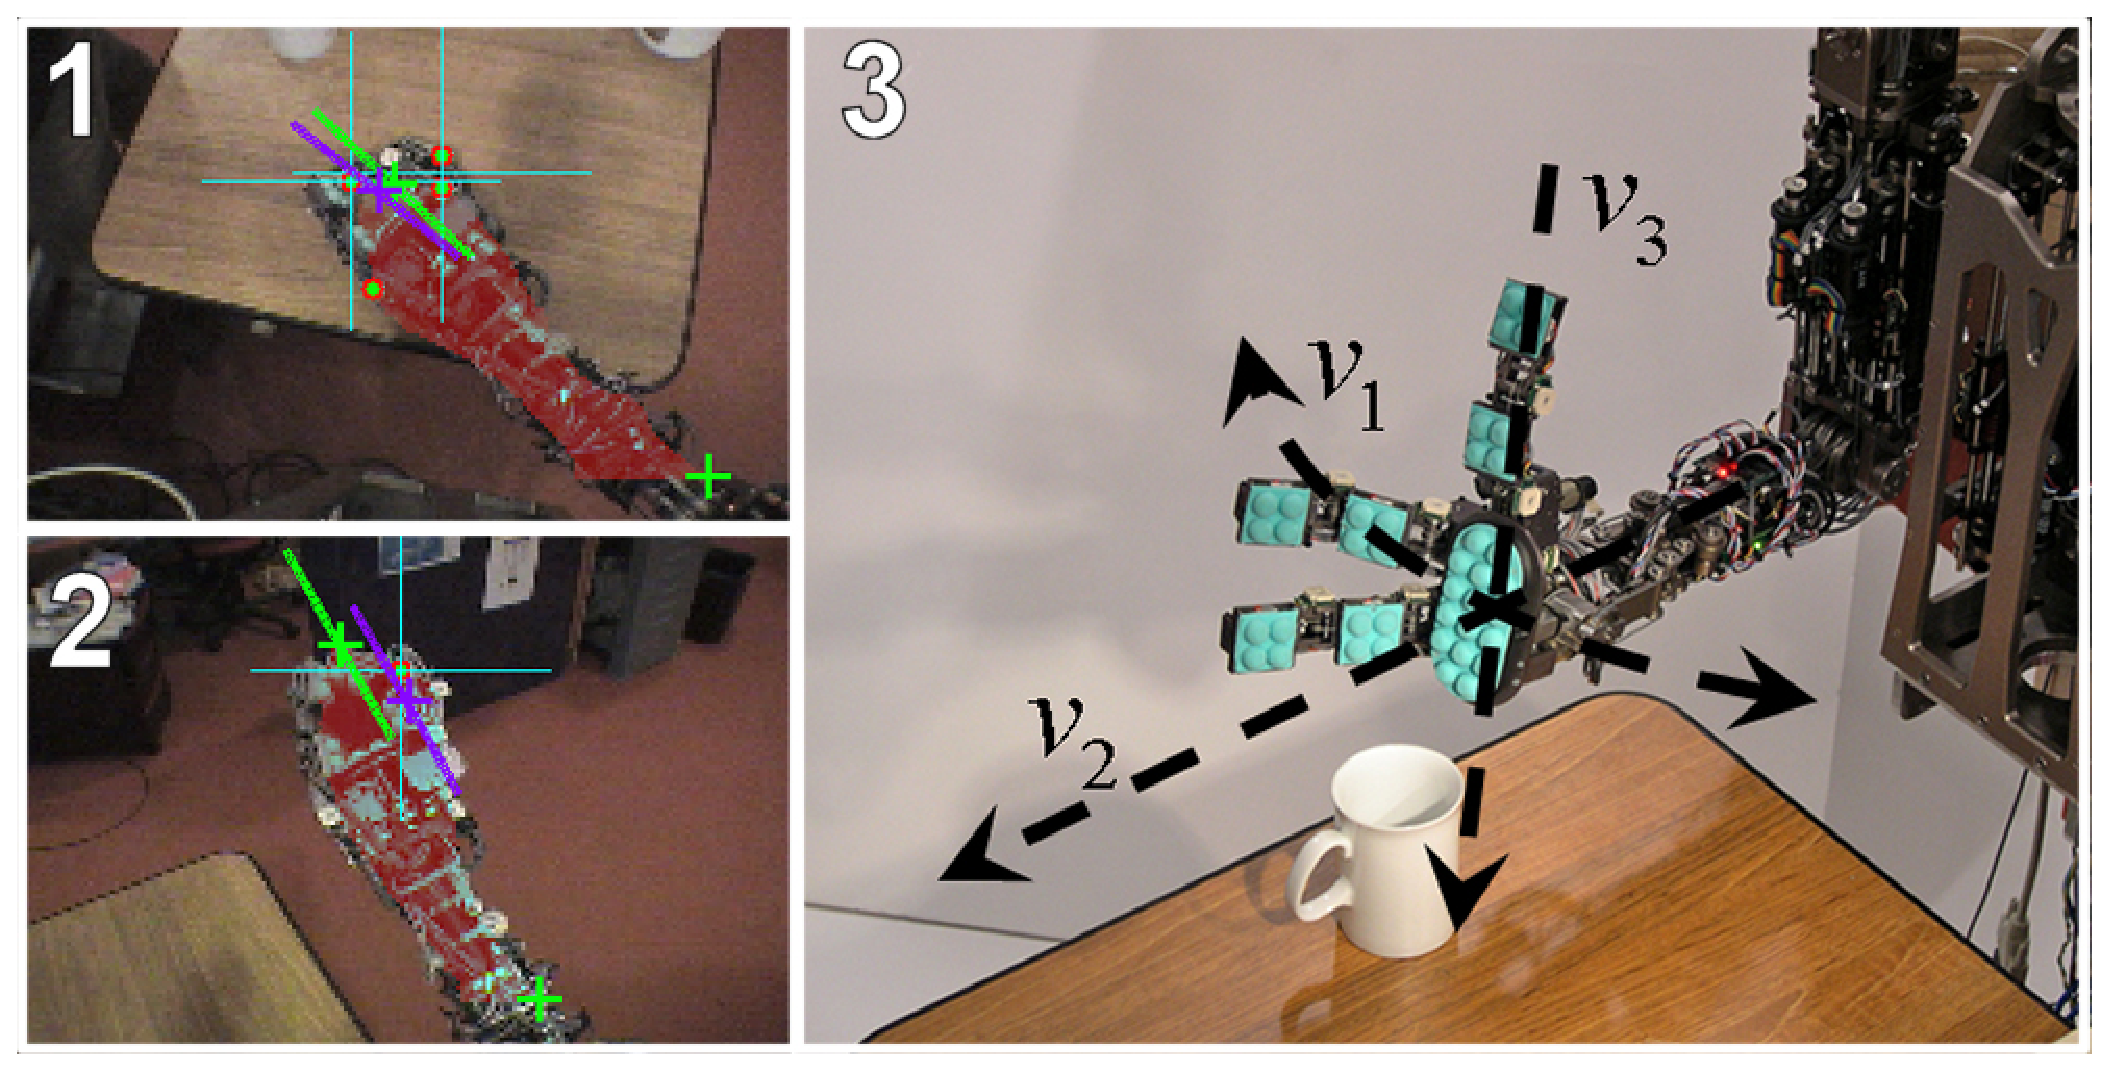
\includegraphics[width=\columnwidth, angle=0 ]{./figures/expl-directions.eps}
  }\caption{Left, frames 1 and 2: hand localization and arm
    orientation. Right, frame 3: exploration primitives. Primitives $v_1$
and $v_2$ are perpendicular and parallel to the arm orientation.
$v_3$ is along the null space of the arm Jacobian. For simpler understanding, 
these primitives are sketched here in the cartesian plane, but 
they are actually computed in the joint space (see 
Section~\ref{sec:controlling} for more details).}
\label{fig:expl-directions}
\end{figure}
%
\subsection{Exploration}
Starting from the direct mapping of the hand position and arm orientation we
can identify a set of explorative primitives, that is a set of vectors in
joint space that allows the robot to explore the arm workspace. We chose three
vectors $v_1$, $v_2$ and $v_3$, as follows (see also 
Figure~\ref{fig:expl-directions}):

$v_1$: moves the hand along the
direction perpendicular to the arm. It is computed by planning a 
reaching movement towards a point a few pixels away from the hand along the
line perpendicular to the orientation of the arm.

$v_2$: moves the hand along the
direction of the arm. It is computed by planning a 
reaching movement towards a point a few pixels away from the hand along the 
arm.

$v_3\in \ker \left(J\left(q_{arm}\right)\right)$: $v_3$ lays in the null 
space of the arm Jacobian; in our case the null space of the Jacobian 
consists of those vector that do not affect
either the projection of the hand onto the visual plane or the orientation
of the arm. These vectors produce a movement of the hand along the optical
axis of the camera, or, in other word, along $R$.
%
\subsection{A grasping behavior}
In this section we describe the grasping behavior of the robot.
The sequence begins when the experimenter waves an object in front
of the robot. The head tracks the object until it remains
stationary within the workspace of the arm. The robot reaches for
the object; motion is planned visually as described in
Section~\ref{sec:reaching}. Reaching is not accurate enough to
guarantee a correct grasp. Since no three dimensional information
is available the arm reaches a region above the object (see
Section~\ref{sec:reaching}). At this point the exploration starts;
the robot computes the explorative primitives $v_1$, $v_2$ and
$v_3$. The exploration uses three behaviors: 
%
\begin{itemize}
%
\item \emph{depth behavior}, moves the hand ``downwards''
along $v_3$; 
%
\item \emph{hovering behavior}, moves the hand back and forth along 
$v_1$;
%
\item \emph{pushing behavior}, moves the hand along $v_2$;
%
\end{itemize}

The \emph{depth behavior} moves the hand along the direction of
the optical axis of the camera and adjusts the height of the hand
with respect to the object/table. To avoid crashing the hand into
the table this behavior is inhibited when the infrared proximity
sensor detects an obstacle (usually this happens close to the
table).
The \emph{hovering behavior} and the \emph{depth behavior} are
activated at the beginning of the exploration. The goal of this
initial phase is to adjust the position of the hand until the
index finger touches the object. This allows adjusting the
position of the hand along the directions $v_1$ and $v_3$. During
the exploration the arm stops when the hand detects the object, to
avoid pushing it away or knocking it over; if no contact is
detected, on the other hand, the amplitude of the exploration is
extended (this increases the probability to touch the object in
case the reaching error is large). The exploration terminates when
the contact with the object is detected by any of the tactile
sensors placed on the index finger. At this point the \emph{hovering
behavior} is suspended and the \emph{pushing behavior} activated. The
``pushing'' movement along $v_2$ brings the palm in contact with
the object while the \emph{depth behavior} takes care of
maintaining the correct distance with the table. When the robot
detects contact on the palm the exploration stops and the
\emph{grasping behavior} is activated. The \emph{grasping
behavior} simply closes the fingers to a specific position. The
low impedance of the joints allows the fingers to adapt to the
different objects being grasped.

Figure \ref{fig:sequence} reports an example of the robot grasping 
a porcelain cup. The grasping behavior proved to be quite reliable, as 
repetitive tests show in Section \ref{sec:results}